
%(BEGIN_QUESTION)
% Copyright 2009, Tony R. Kuphaldt, released under the Creative Commons Attribution License (v 1.0)
% This means you may do almost anything with this work of mine, so long as you give me proper credit

Explain how the following dip tube system measures the {\it density} of the liquid inside the vessel rather than the {\it level}.  Assume the liquid level never drops below the upper dip tube, and that the difference in height between the two dip tubes is fixed at 12 inches (1 foot):

$$\includegraphics[width=15.5cm]{i00264x01.eps}$$

Furthermore, calculate the differential pressure sensed by the DP transmitter for a liquid with a density of 58 pounds per cubic foot.

\vfil 

\underbar{file i00264}
\eject
%(END_QUESTION)





%(BEGIN_ANSWER)

This is a graded question -- no answers or hints given!

%(END_ANSWER)





%(BEGIN_NOTES)

So long as both dip tubes remain submerged, the only variable affecting dip tube differential pressure is liquid density (since the height difference between the two tubes is fixed).

\vskip 10pt

Pressure = 11.15 inches water column (0.4028 PSID) at a liquid density of 58 lb/ft$^{3}$.

%INDEX% Measurement, density: bubble tube (bubbler)
%INDEX% Measurement, density: dip tube (bubbler)
%INDEX% Measurement, density: hydrostatic pressure

%(END_NOTES)


